%File: cylinder.tex
%Author: Yuxin Wu <ppwwyyxx@gmail.com>

\section{Cylinder Mode}
\label{sec:cylinder}
\subsection{Necessity of Projection}
If a rotational input is given, as most panoramas are built,
using planar homography leads to \textbf{vertical distortion}, such as \figref{distort}.
\begin{figure}[H]
  \centering
  \includegraphics[width=0.9\textwidth]{res/distort.png}
  \caption{Vertical Distortion with Homography on a Planar\label{fig:distort}}
\end{figure}

This is because a panorama is essentially an image taken with
a cylindrical or spherical lens, not a planar lens any more.
Under this circumstance, a circle around the camera (in \figref{distort}) should
become a line.

There are two ways to handle with this problem: to warp before or after
transform estimation.
\footnote{A good app revealing the reason of this projection can be seen at \url{http://graphics.stanford.edu/courses/cs178-12/applets/projection.html}}
These are the two modes used in this system. In this section we will
introduce the algorithms used in cylinder mode.

\subsection{Warp}
One way of doing this is to project each image
to a cylinder surface at the beginning, by the following formula:

\[  \begin{cases}
    x' = \arctan{\dfrac{x-x_c}{f}}\\
    y' = \dfrac{y-y_c}{\sqrt{(x-x_c)^2 + f^2}}
  \end{cases}\]
where $ f$ is the focal length of the camera, and $ x_c, y_c$ is the center of image.
See \verb|stitch/warp.cc|

After projecting all images to the cylinder surface, images can be
simply stitched together by an affine transformation.
The result is in shown in \figref{cyl}. Note that the white line on
the ground is straightened.
\begin{figure}[H]
  \centering
  \begin{minipage}[b]{0.24\linewidth}
    \includegraphics[scale=0.3]{res/1.png}
  \end{minipage}
  \begin{minipage}[b]{0.24\linewidth}
    \includegraphics[scale=0.3]{res/2.png}
  \end{minipage}
  \begin{minipage}[b]{0.24\linewidth}
    \includegraphics[scale=0.3]{res/3.png}
  \end{minipage}
  \begin{minipage}[b]{0.24\linewidth}
    \includegraphics[scale=0.3]{res/4.png}
  \end{minipage}

  \includegraphics[width=0.9\textwidth]{res/warped_stitch.png}
  \caption{Stitching Result After Projection\label{fig:cyl}}
\end{figure}

\subsection{Straightening}
\begin{figure}[H]
  \centering
  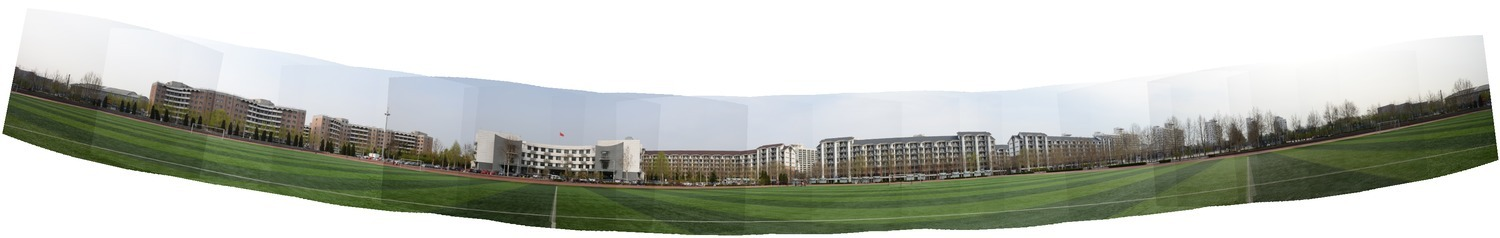
\includegraphics[width=\textwidth]{res/bend.jpg}
  \caption{Bended Panorama\label{fig:bend}}
\end{figure}

Since the tilt angle of camera is unknown,
the projection to the cylinder could still lead to distortion.
Then the output panorama would be bended as shown in \figref{bend}.
Instead of using the first image as the pivot, and calculating all the other transformation relative to it,
using the image in the middle as the pivot can help reduce the tilt effect.
Apart from that, I found a method to reduce the effect, by searching for $ y_c$
in the above warping formula.

Since the effect is caused by camera tilt, $ y_c$ could differ from $ \dfrac{height}{2}$.
The algorithm works by changing $ y_c$ and find a value which leads to the most straight result. See \verb|Stitcher::update_h_factor()|.
After this processes, the result is like \figref{unbend}.

\begin{figure}[H]
  \centering
  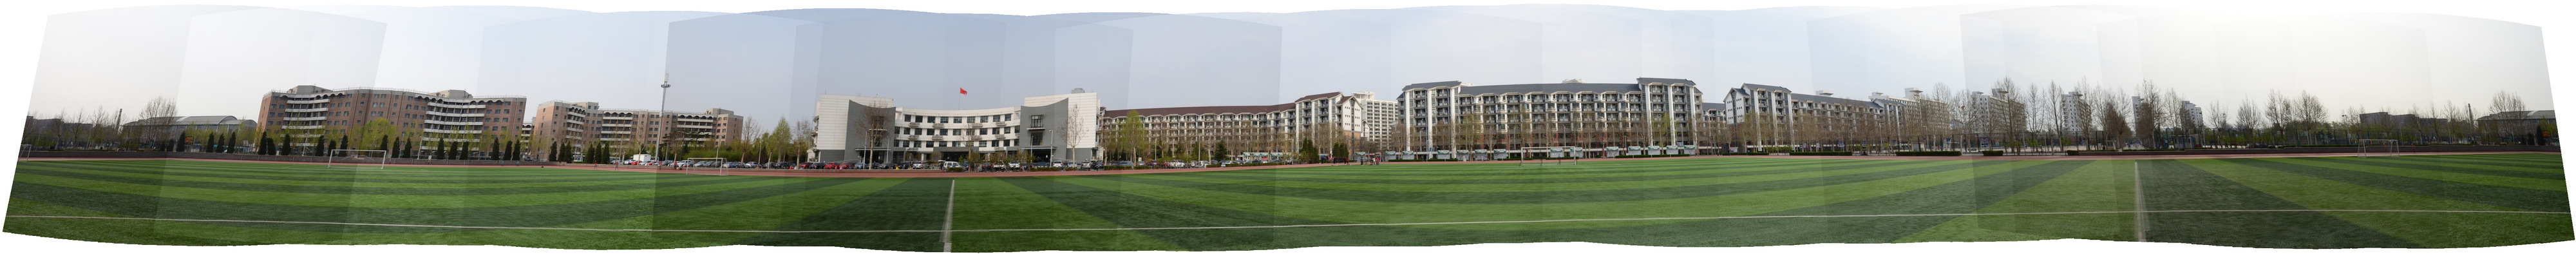
\includegraphics[width=\textwidth]{res/unbend.jpg}
  \caption{After bend correction\label{fig:unbend}}
\end{figure}

The change of $y_c$ is not enough, since we are still warping
images to a vertical cylinder.
The error can be seen at the left and right edges in \figref{unbend}.
To account for this error, I used a perspective transform
to align the left and right edges (\verb|Stitcher::perspective_correction|). The result is in \figref{unbend-persp}
\begin{figure}[H]
  \centering
  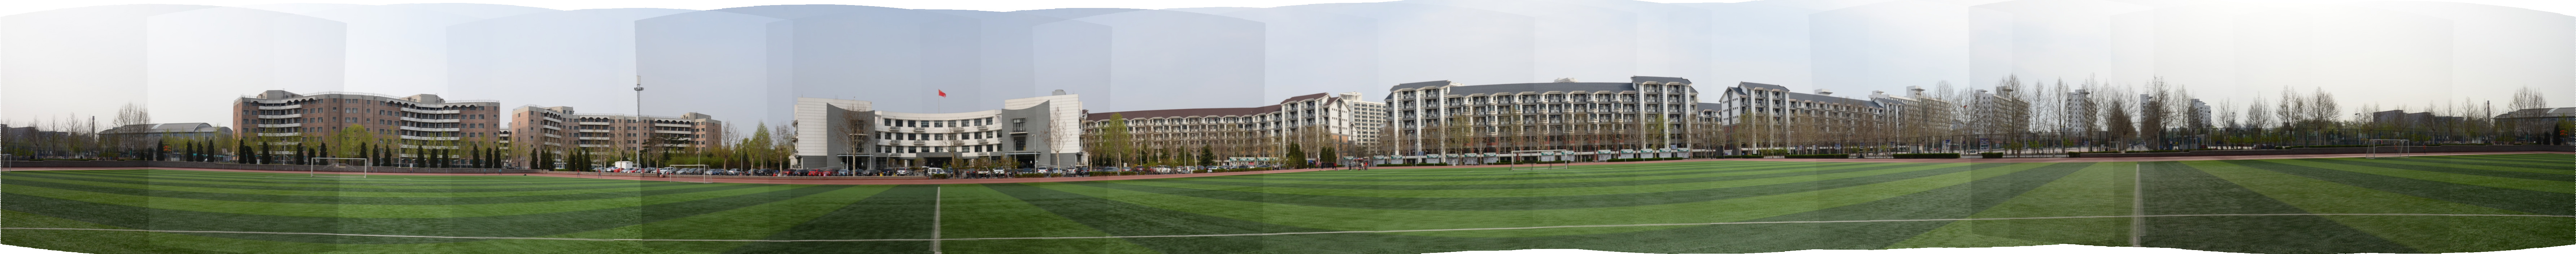
\includegraphics[width=\textwidth]{res/unbend-persp.jpg}
  \caption{After perspective correction \label{fig:unbend-persp}}
\end{figure}

